\documentclass[a4paper,11pt,french]{article}
\usepackage[utf8]{inputenc}

\usepackage[T1]{fontenc}
\usepackage[francais]{babel} 
\usepackage[top=2cm, bottom=2cm, left=2cm, right=2cm, includeheadfoot]{geometry} %pour les marges
\usepackage{lmodern}
\usepackage{pict2e}
\usepackage{fancyhdr} % Required for custom headers
\usepackage{lastpage} % Required to determine the last page for the footer
\usepackage{extramarks} % Required for headers and footers
\usepackage{graphicx} % Required to insert images
\usepackage{tabularx, longtable}
\usepackage{color, colortbl}
\usepackage{lscape}
%\usepackage[hidelinks]{hyperref}
\usepackage{longtable}
\usepackage{multirow}
\usepackage{rotating}
%\usepackage{pgfgantt}
%\usepackage{pgfcalendar}
%\usepackage{ifthen}
\usepackage{gensymb}



\linespread{1.1} % Line spacing

% Set up the header and footer
\pagestyle{fancy}
\lhead{\textbf{\hmwkClass -- \hmwkSubject \\ \hmwkTitle \\ \hmwkDocName}} % Top left header
\rhead{
\includegraphics[width=10em]{../images/logo_univ.png}}
\lfoot{\lastxmark} % Bottom left footer
\cfoot{} % Bottom center footer
\rfoot{Page\ \thepage\ / \pageref{LastPage}} % Bottom right footer
\renewcommand\headrulewidth{0.4pt} % Size of the header rule
\renewcommand\footrulewidth{0.4pt} % Size of the footer rule

\setlength{\headheight}{40pt}

\newcommand{\hmwkTitle}{Transchiffrement} % Assignment title
\newcommand{\hmwkClass}{Master 2 SSI } % Course/class
\newcommand{\hmwkAuthorName}{Emile GÉNÉRAT} % Your name
\newcommand{\hmwkSubject}{Conduite de projet} % Subject
\newcommand{\hmwkDocName}{Plan de Développement} % Document name

\newcommand{\version}{1.1} % Document version
\newcommand{\docDate}{22 Janvier 2014} % Document date
\newcommand{\checked}{Jean-Baptiste SOUCHAL} % Checker name
\newcommand{\approved}{} % Approver name

\makeatletter
\newcommand{\resettranslate}{\let\translate\@firstofone}
\makeatother

\definecolor{gris}{rgb}{0.95, 0.95, 0.95}

\title{
\vspace{2in}
\textmd{\textbf{\hmwkClass :\ \hmwkTitle}}\\
\normalsize\vspace{0.1in}\small{Due\ on\ \hmwkDueDate}\\
\vspace{0.1in}\large{\textit{\hmwkClassInstructor\ \hmwkClassTime}}
\vspace{3in}
}

\author{\hmwkAuthorName}
\date{} % Insert date here if you want it to appear below your name


\usepackage{amsmath}
\begin{document}
\newcount\startdate
\newcount\daynum
%\pgfcalendardatetojulian{2013-01-021}{\startdate}
\pagestyle{fancy}

\vspace*{5cm}
\begin{center}\textbf{\Huge{\hmwkDocName}}\end{center}
\vspace*{4.5cm}
	

\fcolorbox{black}{gris}{
\begin{minipage}{15cm}
\begin{tabularx}{10cm}{lXl}
	\bfseries{Version} & & \version\\
	& & \\
	\bfseries{Date} & & \docDate\\
	& & \\
	\bfseries{Rédigé par} & & \hmwkAuthorName \\
	& & \\
	\bfseries{Relu par} & & \checked \\
	& & \\
	\bfseries{Approuvé par} & & \approved \\
	& & \\
\end{tabularx}
\end{minipage}
}

\newpage

%Tableau de mises à jour
\vspace*{1cm}
\begin{center}
\textbf{\huge{Versions}}\\
\vspace*{3cm}
	\begin{tabularx}{16cm}{|c|c|X|}
	\hline
	\bfseries{Version} & \bfseries{Date} & \bfseries{Modifications réalisées}\\
	\hline
	1.0 & 13/12/2013 & Création\\
	\hline
	1.1 & 22/01/2014 & Modification pour prise en compte des remarques du Client et de l'audit \\
	\hline
	\end{tabularx}
\end{center}

%La table des matières
\clearpage
\tableofcontents
\clearpage
\newpage
\section{Contexte du projet}


Pour garantir la confidentialité du trafic internet, les sites ont de plus en plus souvent recours au chiffrement des échanges. Ce chiffrement s'effectue de bout en bout, du client jusqu'au serveur.
Ainsi, un intrus qui intercepte les connexions ne peut pas lire les paquets qui transitent.


Fréquemment, les entreprises analysent le trafic entrant et sortant de leur réseau. Cette analyse du contenu des paquets permet par exemple de chercher la présence de virus.


Le but du projet est de fournir une solution de transchiffrement, qui permette d'analyse en clair au sein du proxy les paquets d'une connexion chiffrée. Pour cela, il faut établir une connexion chiffrée vers le client, et une autre vers le serveur distant.


Pour cela, nous aurons besoin d'une autorité de certification reconnue par le client pour générer des certificats.
Il existe plusieurs méthodes, dont l'étude des collisions MD5.
Le but de la collision revient à générer un deuxième certificat dont la clé publique est différente, mais qui a la même signature MD5.


\subsection{Respect de la législation en vigueur}
\begin{itemize}

\item Le résultat du projet ne doit pas faire l'objet d'une utilisation illégale
\item Le dispositif ne peut être utilisé qu'avec l'accord explicite du propriétaire du réseau
\item La surveillance du trafic ne peut être faite sans le consentement des utilisateurs
\end{itemize}
\newpage
\section{Documents de référence}

\begin{itemize}
\item Étude et mise en oeuvre de solutions de Transchiffrement SSL/TLS : sujet\_projet\_ssi.pdf
\item Spécification Technique du besoin : STB\_v1.1.pdf
\item Architecture Logicielle : DAL\_v1.1.pdf
\item Cahier des Recettes : CDR\_v1.1.pdf
\item Analyse des risques : ADR\_v1.1.pdf
\item Plan de développement : PDD\_v1.1.pdf
\end{itemize}

\newpage
\section{Terminologie et sigles utilisés}

\begin{description}
\item[SSL] Secure Sockets Layer
\item[TLS] Transport Layer Security (remplace SSL)
\item[HTTPS] Hypertext Transfer Protocol Secure
\item[MD5] Message-digest algorithm
\item[AC] Autorité de Certification
\end{description}

%\newpage
%\section{Méthodologie de développement}

\newpage
\section{Organisation et responsabilités}

\begin{itemize}
\item Les développeurs : Tous les membres du projets sont en charge de la production de l'application, ainsi que des recherches sur les collisions de certificats.

\item Relation client : Julien BOURDON est en charge du suivi de la relation client. Il doit s'assurer de l'adéquation du travail réalisé par le groupe, par rapport aux besoins exprimés par le client.

\item Le responsable qualité : Jean-Baptiste SOUCHAL s'occupe de tester les fonctionnalités du produit final. C'est lui qui s'assure que les fonctionnalités développées sont conformes aux spécifications.

\item Le chef de projet : Emile GÉNÉRAT rend compte de l'évolution du projet. De plus il s'assure du bon fonctionnement du travail d'équipe, au niveau de la communication et du suivi des rôles de chacun.
\end{itemize}

\begin{figure}[h!]
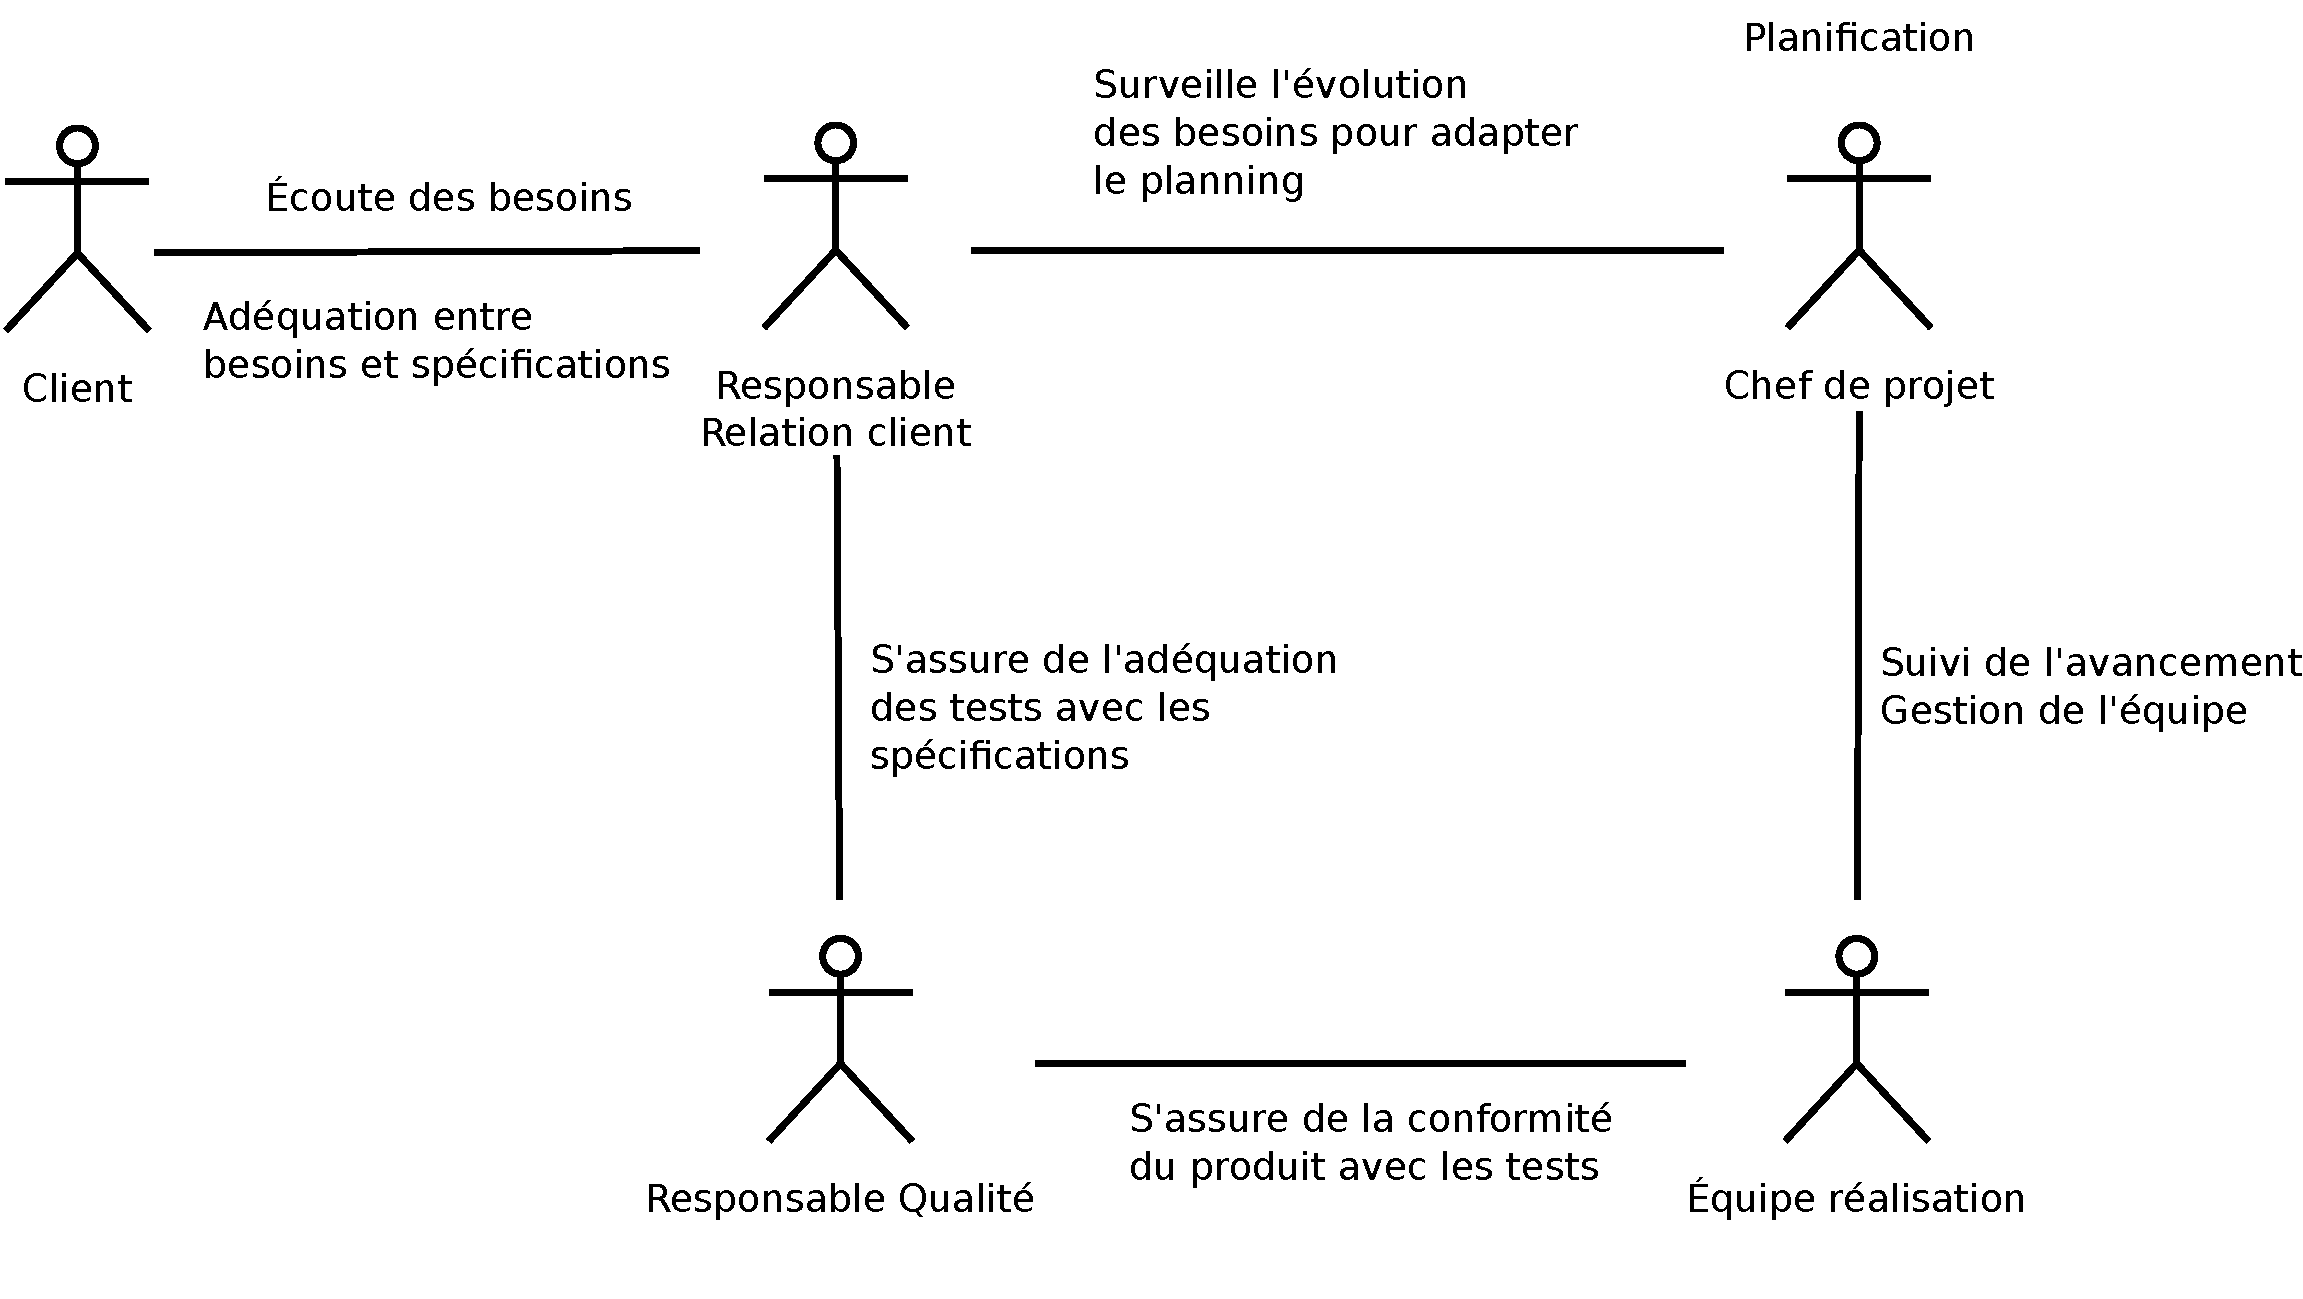
\includegraphics[width=\textwidth]{images/interaction_acteurs.pdf}
\end{figure}


%\newpage
%\section{Organigramme des tâches}
\newpage
\section{Lotissement}

Les fonctionnalités finales attendues sont :
\begin{itemize}
\item une application servant de proxy  
\item un dossier de recherche sur les collisions MD5, ainsi qu'une mise en oeuvre.
\end{itemize}

Chaque fonctionnalité fait l'objet d'une livraison au client, pour prendre en compte ses remarques.

La livraison finale des deux lots est prévue pour le 21 février.

\newpage
\section{Dimensionnement des moyens}

\begin{itemize}
\item 5 étudiants avec un ordinateur chacun
\item Un serveur dédié au calcul de collisions.
\end{itemize}

\subsection{Description des tâches}

Le lotissement n'est pas définitif. Le projet contient deux parties principales, qui doivent être développées parallèlement.

Développement d'un proxy applicatif.
\begin{itemize}
\item Génération d'un certificat signé par une autorité reconnue
\item Installation et acceptation de l'autorité sur le client
\item Établissement d'une connexion chiffrée ou non
\item Transchiffrement des paquets
\end{itemize}
Recherche de collisions de certificats.
\begin{itemize}
\item Lecture des documents
\item Étude de la faisabilité d'une collision
\item Développement d'une application qui permette de rechercher une seconde pré-image.
\item Mise en production d'un programme de recherche de collisions, sur une machine mise à notre disposition.
\end{itemize}

\subsection{Évaluation des charges et répartition des tâches}

\begin{itemize}
\item Le temps de travail total est de 35h * 6 semaines * 5 personnes, soit 1050 heures.
\item Charge totale des tâches du projet : 990h
\item Charge totale des réunions : 6 * 5 * 2 = 60h
\item Charge total du projet : 1050h
\end{itemize}

\newpage
\begin{figure}[h!]
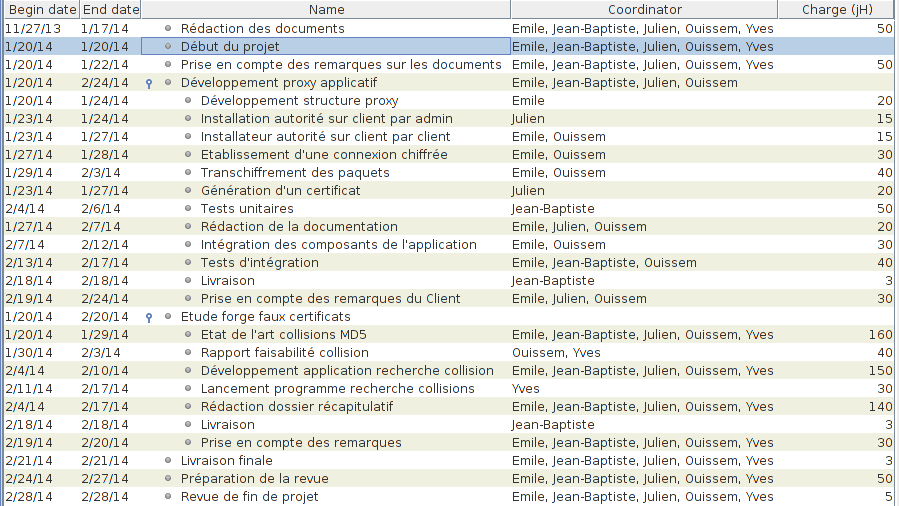
\includegraphics[width=\textwidth]{images/taches.png}
\end{figure}

\newpage
\begin{figure}[h!]
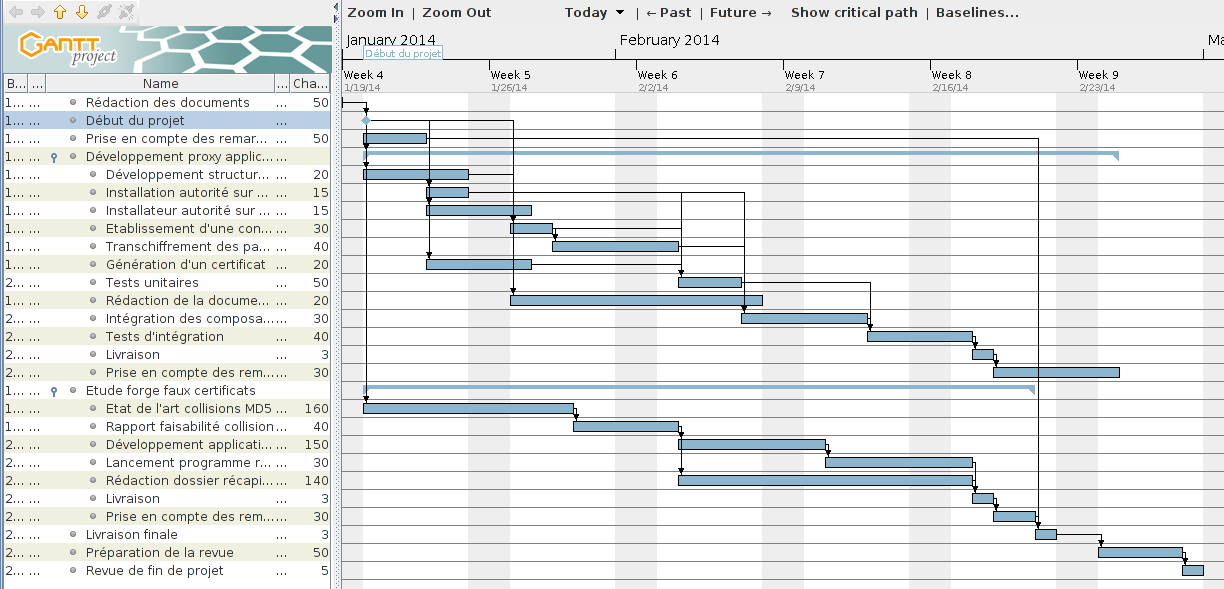
\includegraphics[width=0.9\textheight, angle=90]{images/planification.png}
\end{figure}





\newpage
\section{Procédés de gestion}
%\subsection{Gestion de la documentation}
%\subsection{Gestion des configurations}

\subsection{Dates clés}
\begin{itemize}
\item Début du projet : 20 janvier 2014
\item Livraisons partielles des sous-lots : 17 février 2014
\item Livraison finale du projet : 21 février 2014
\item Revue de fin de projet : 28 février 2014
\end{itemize}

\newpage
\section{Procédures de suivi d'avancement}

Chaque semaine, l'équipe se réunit pour évaluer l'avancement des tâches.
Chaque membre de l'équipe présente l'avancement des tâches qui lui ont été affectées.
Cette réunion permet d'établir un avancement global du projet.
C'est dans cette réunion que les ajustements éventuels du planning sont décidés, en accord avec le client.


\end{document}